\newpage
\section{Triển khai}
\subsection{Sơ đồ tổng quan}
\begin{figure}[H]
    \centering
    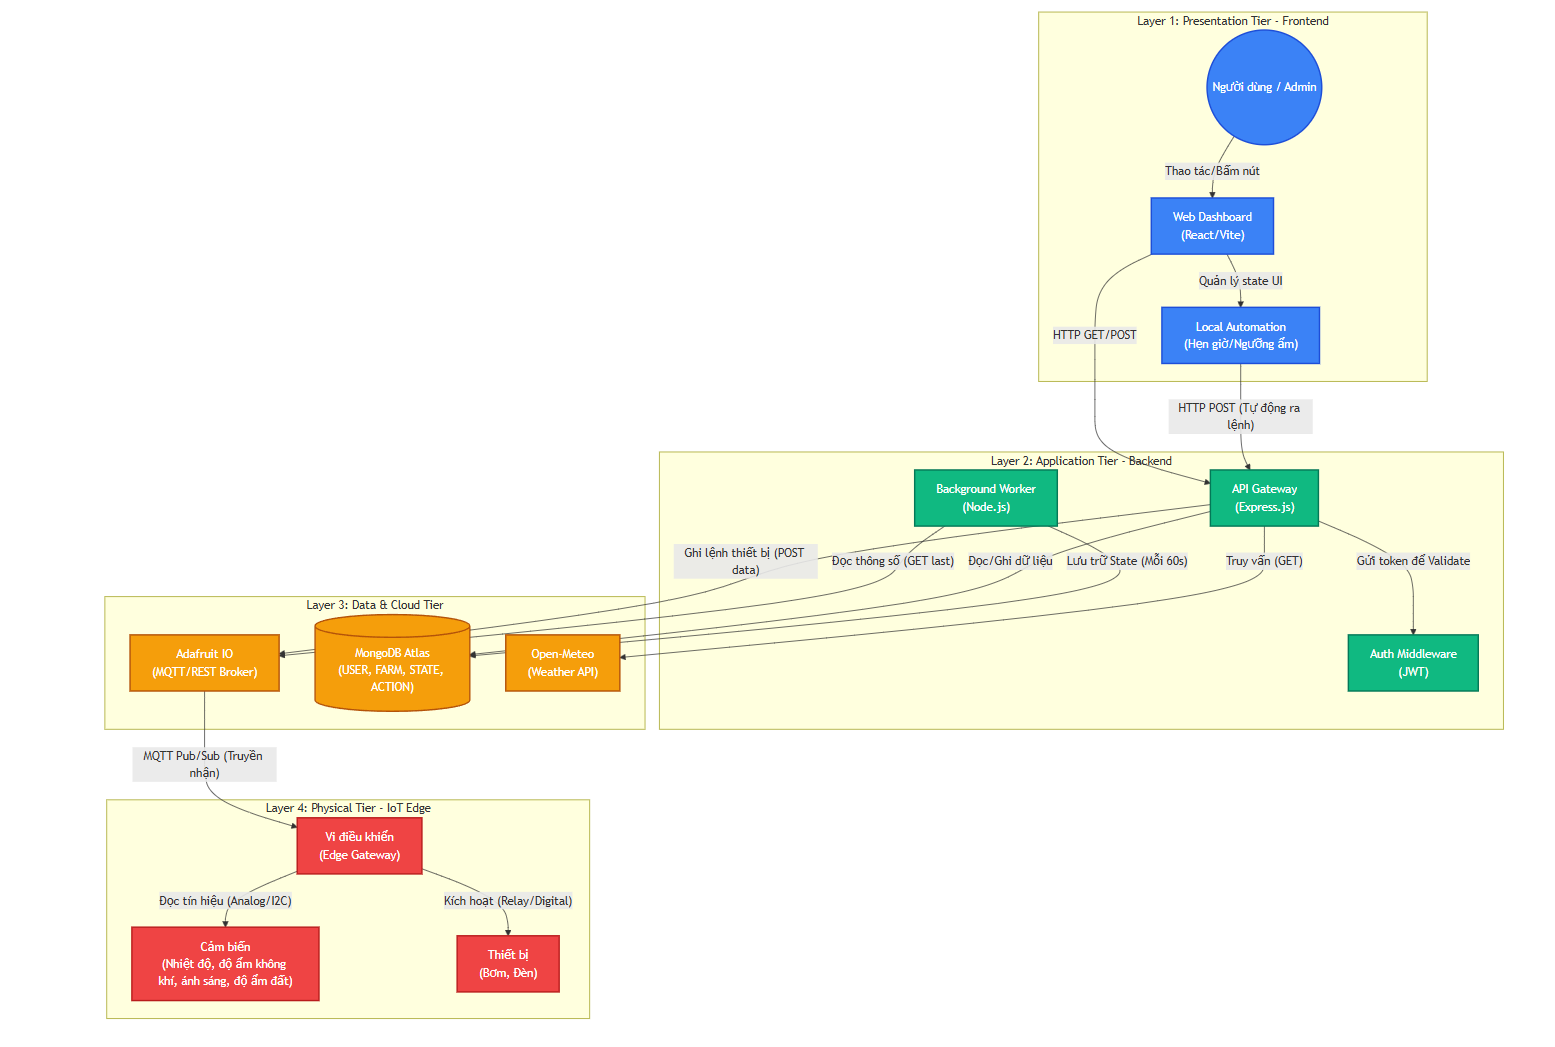
\includegraphics[width=0.8\textwidth]{img/sodo.png}
    \caption{Sơ đồ tổng quan kiến trúc hệ thống}
\end{figure}

\subsection{Kiến trúc tổng thể}
Hệ thống gồm 4 phần chính:
\begin{itemize}
  \item \textbf{Frontend}: Ứng dụng SPA (Single Page Application) viết bằng ReactJS, tương tác với
backend thông qua REST API. Giao diện người dùng cho phép giám sát và điều khiển các
thiết bị IoT
  \item \textbf{Backend}: Phần mềm phía máy chủ viết bằng Node.js, xử lý logic ứng dụng, quản lý cơ sở dữ liệu và cung cấp REST API cho frontend.
  \item \textbf{Cơ sở dữ liệu}:  MongoDB: Lưu trữ dữ liệu phi cấu trúc và thời gian thực (log thiết bị, dữ liệu cảm
biến,...).
  \item \textbf{Hệ thống IoT}: \begin{itemize}
    \item Sử dụng Yolo:Bit và bộ AIoT Kit do OhStem phát triển
    \item Thiết bị giao tiếp với server qua các giao thức HTTP, MQTT, và đồng bộ thời gian với
NTP
\item Thiết bị gửi dữ liệu cảm biến và nhận lệnh điều khiển từ backend hoặc trực tiếp từ giao
diện người dùng
  \end{itemize}
  
\end{itemize}

Hệ thống được xây dựng theo mô hình Client-Server nhằm tách biệt rõ ràng giữa giao
diện người dùng và phần xử lý phía máy chủ. Cấu trúc này không chỉ giúp tối ưu hiệu suất
mà còn đảm bảo khả năng phát triển và mở rộng hệ thống trong tương lai.
\begin{itemize}
    \item Client: Là phần giao diện tương tác trực tiếp với người dùng. Nó chịu trách nhiệm thu
thập đầu vào (input), hiển thị dữ liệu (output) và gửi yêu cầu đến server thông qua các
API.
    \item Server: Đảm nhiệm các chức năng xử lý nghiệp vụ, quản lý cơ sở dữ liệu và phản hồi
các yêu cầu từ client. Giao tiếp giữa client và server sử dụng chuẩn RESTful API.
Ưu điểm của mô hình này là khả năng mở rộng linh hoạt (scalability) và dễ bảo
trì (maintainability), khi client và server có thể phát triển độc lập, triển khai ở các
nền tảng khác nhau và nâng cấp mà không ảnh hưởng lẫn nhau.
\end{itemize}


\subsection{Demo}
\begin{itemize}
  \item \textbf{Link source code on GitHub}: \href{https://github.com/huonglandoan/Smartfarm}{https://github.com/huonglandoan/Smartfarm}
  \item \textbf{Link video demo:} \href{https://youtu.be/-sP-Kj_6f_g}{Video demo}
\end{itemize}
